Here we describe the second prototype of GEA with all the modifications, additions and new implementations coming from the feedbacks and results of the first evaluation.\\
For what concerns the requirements, goals, needs, target group, contexts and constraints refers to \autoref{chap:first-prot} because they remained the same. Also the UX design of the three mini-game in virtual reality is the same as in the cited chapter except for minimal modifications reported in the following sections.\\
The new home page of GEA is now the one reported in Figure \ref{fig:newhomepage}. Here the user can choose if he/she wants to play in virtual reality mode or in touchscreen mode. \\
\begin{figure}[H]
\centering
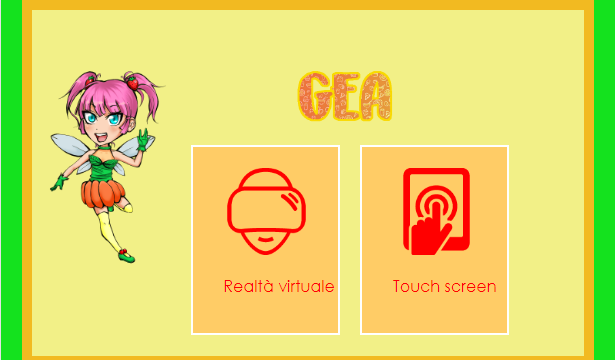
\includegraphics[width=10cm, height=6cm]{immagini/homepagenew.png}
\caption{Home page: second prototype}\label{fig:newhomepage}
\end{figure}
In figure \ref{fig:newselection} we show the new page for selecting the mini-game, here the user can choose between four games: "Lear with the pyramid!", "Healthy or not?", "Let's eat!" and "Find the allergen!". This page is the same for virtual reality and touchscreen.
\begin{figure}[H]
\centering
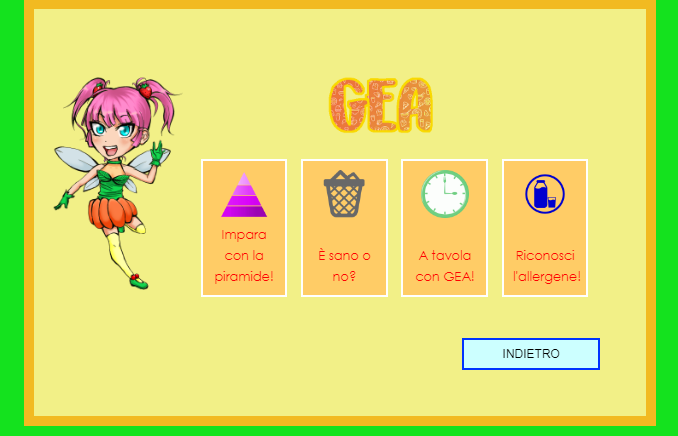
\includegraphics[width=10cm, height=6cm]{immagini/selectionnew.png}
\caption{Page for selecting the mini-game: second prototype}\label{fig:newselection}
\end{figure}
After having chosen the game the next page will be for the selection of the difficulty level, this page is the same as the first prototype and for every game.
\section{Touchscreen}
In this section with show the screenshots abouto the touchscreen part of GEA.\\
First of all we want to impose to use the smartphone or better the tablet in the landascape mode so if the user is playing in portrait mode appears the allert message in Figure \ref{fig:rotate}.\\
We have decided to do that to improve the game experience because in the portrait mode all the objects, and so the foods, are too small and we cannot represent a real room. If the user saves the game on the device the rotation will be authomatic because of the manifest we have written but when you play on a browser this is not possible.\\
Also during the session if the user rotates the device the game stops and the message appears then when you come back to the landscape mode you can play exactly from that moment and not from the beginning.
\newpage
\begin{figure}[H]
\centering
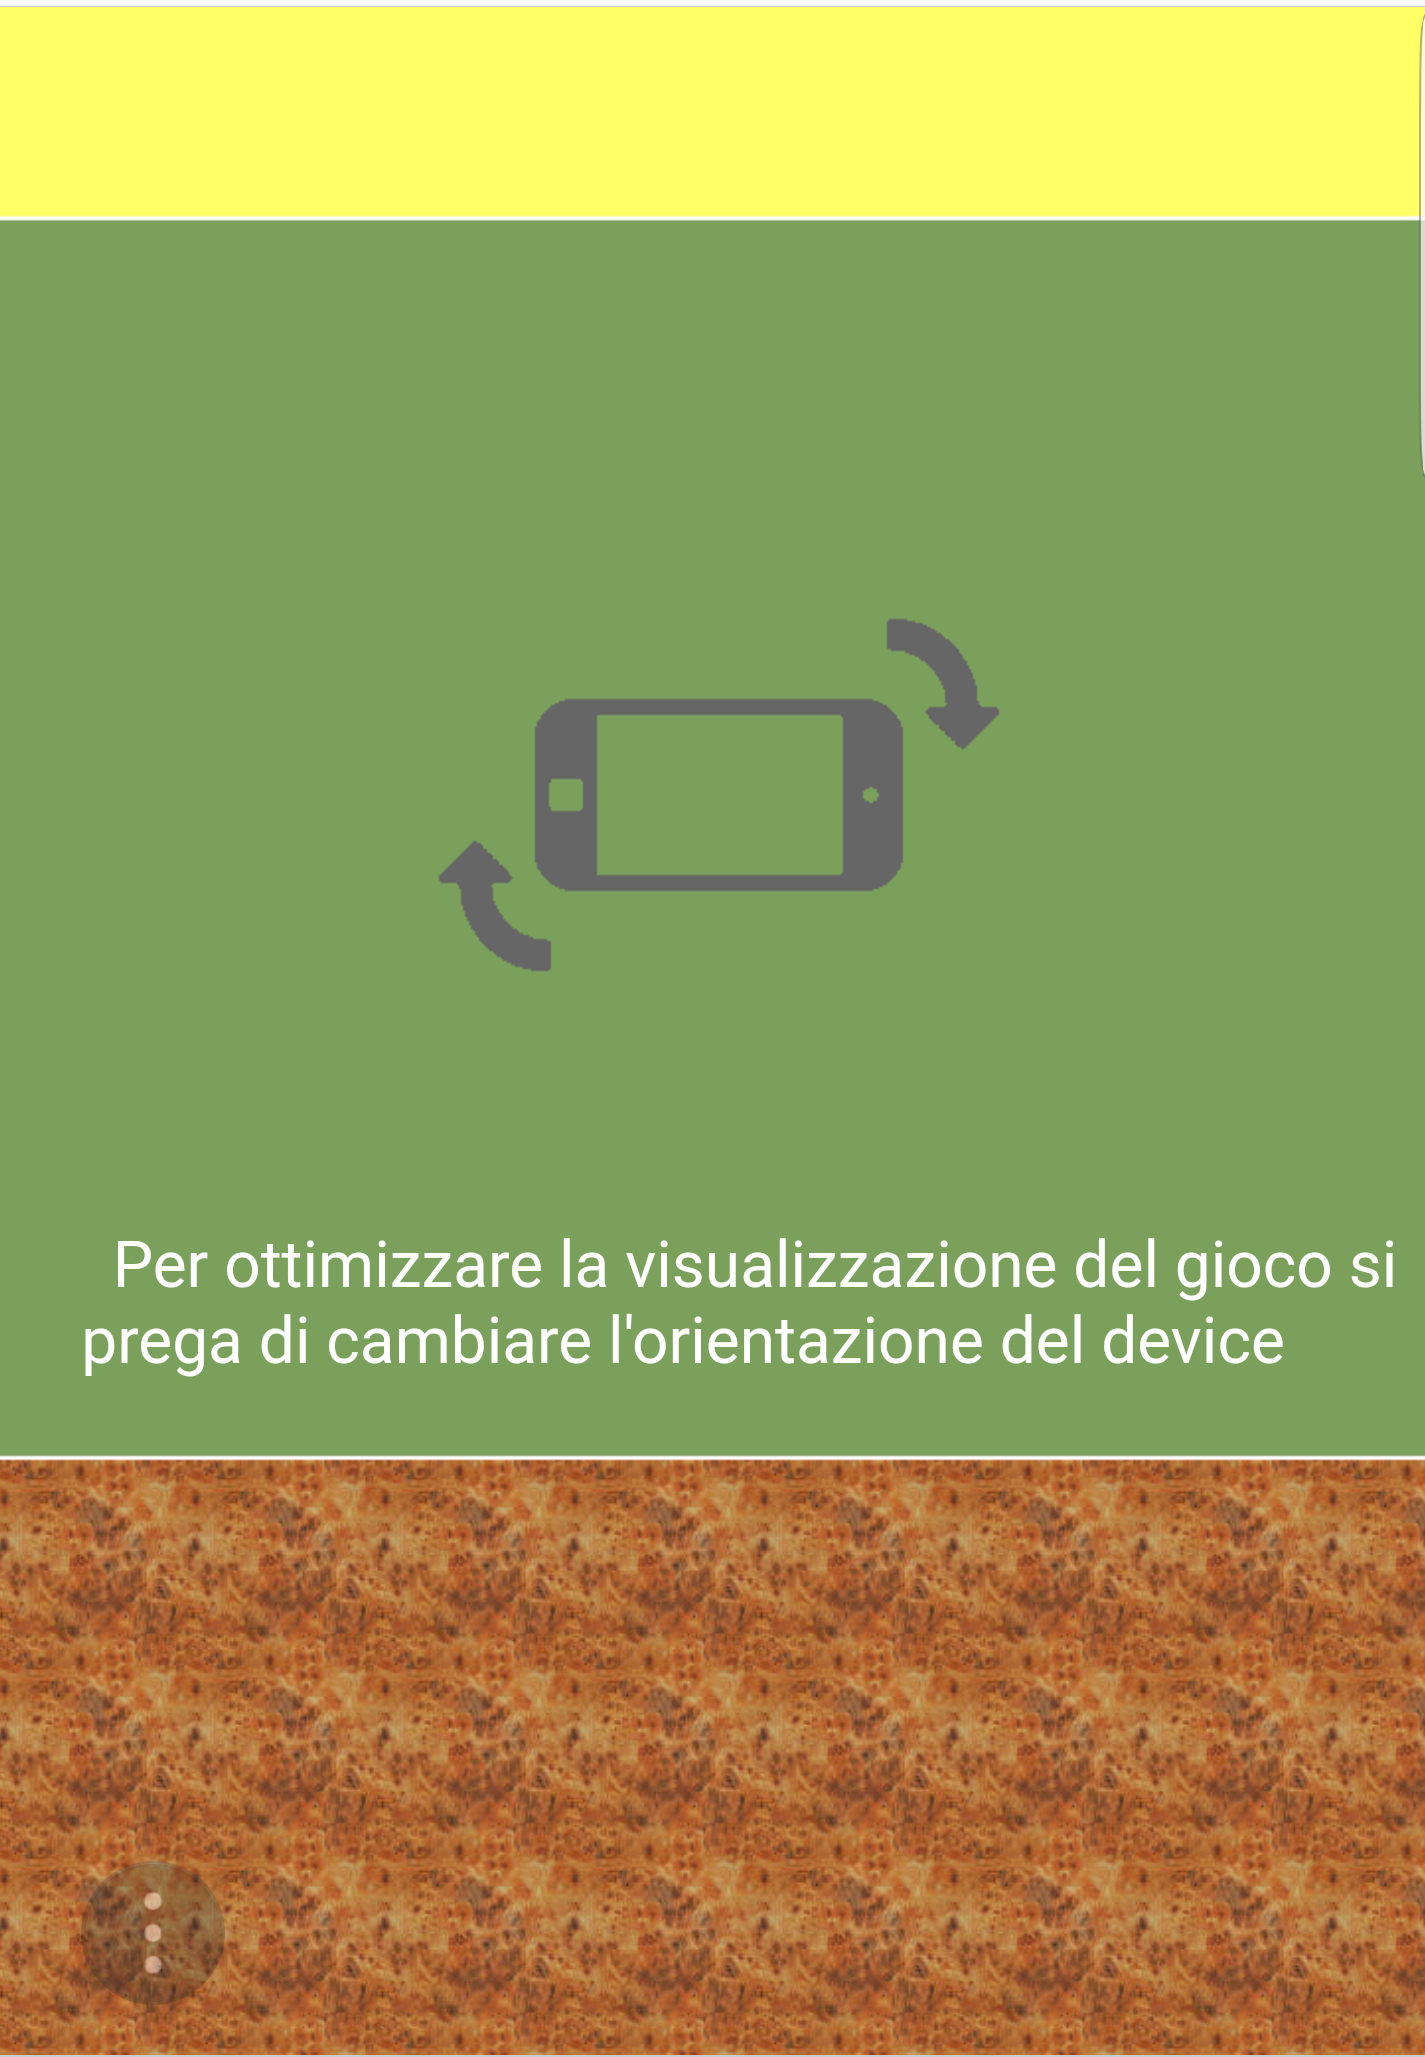
\includegraphics[width=6cm, height=10cm]{immagini/rotate.png}
\caption{Screenshot of rotate message}\label{fig:rotate}
\end{figure}
For what concerns the logic the mini-games are remained the same, the only things that are changed are the graphic (not 3D dimensions but 2D dimensions) and the interaction (not looking at something but touching something).\\
In the following we can see the screenshots about "Learn with the pyramid!" (Figure \ref{fig:newpyramid}), "Healthy or not?" (Figure \ref{fig:newhealthy}) and "Let's eat!" (Figure \ref{fig:newlet}).
\begin{figure}[H]
\centering
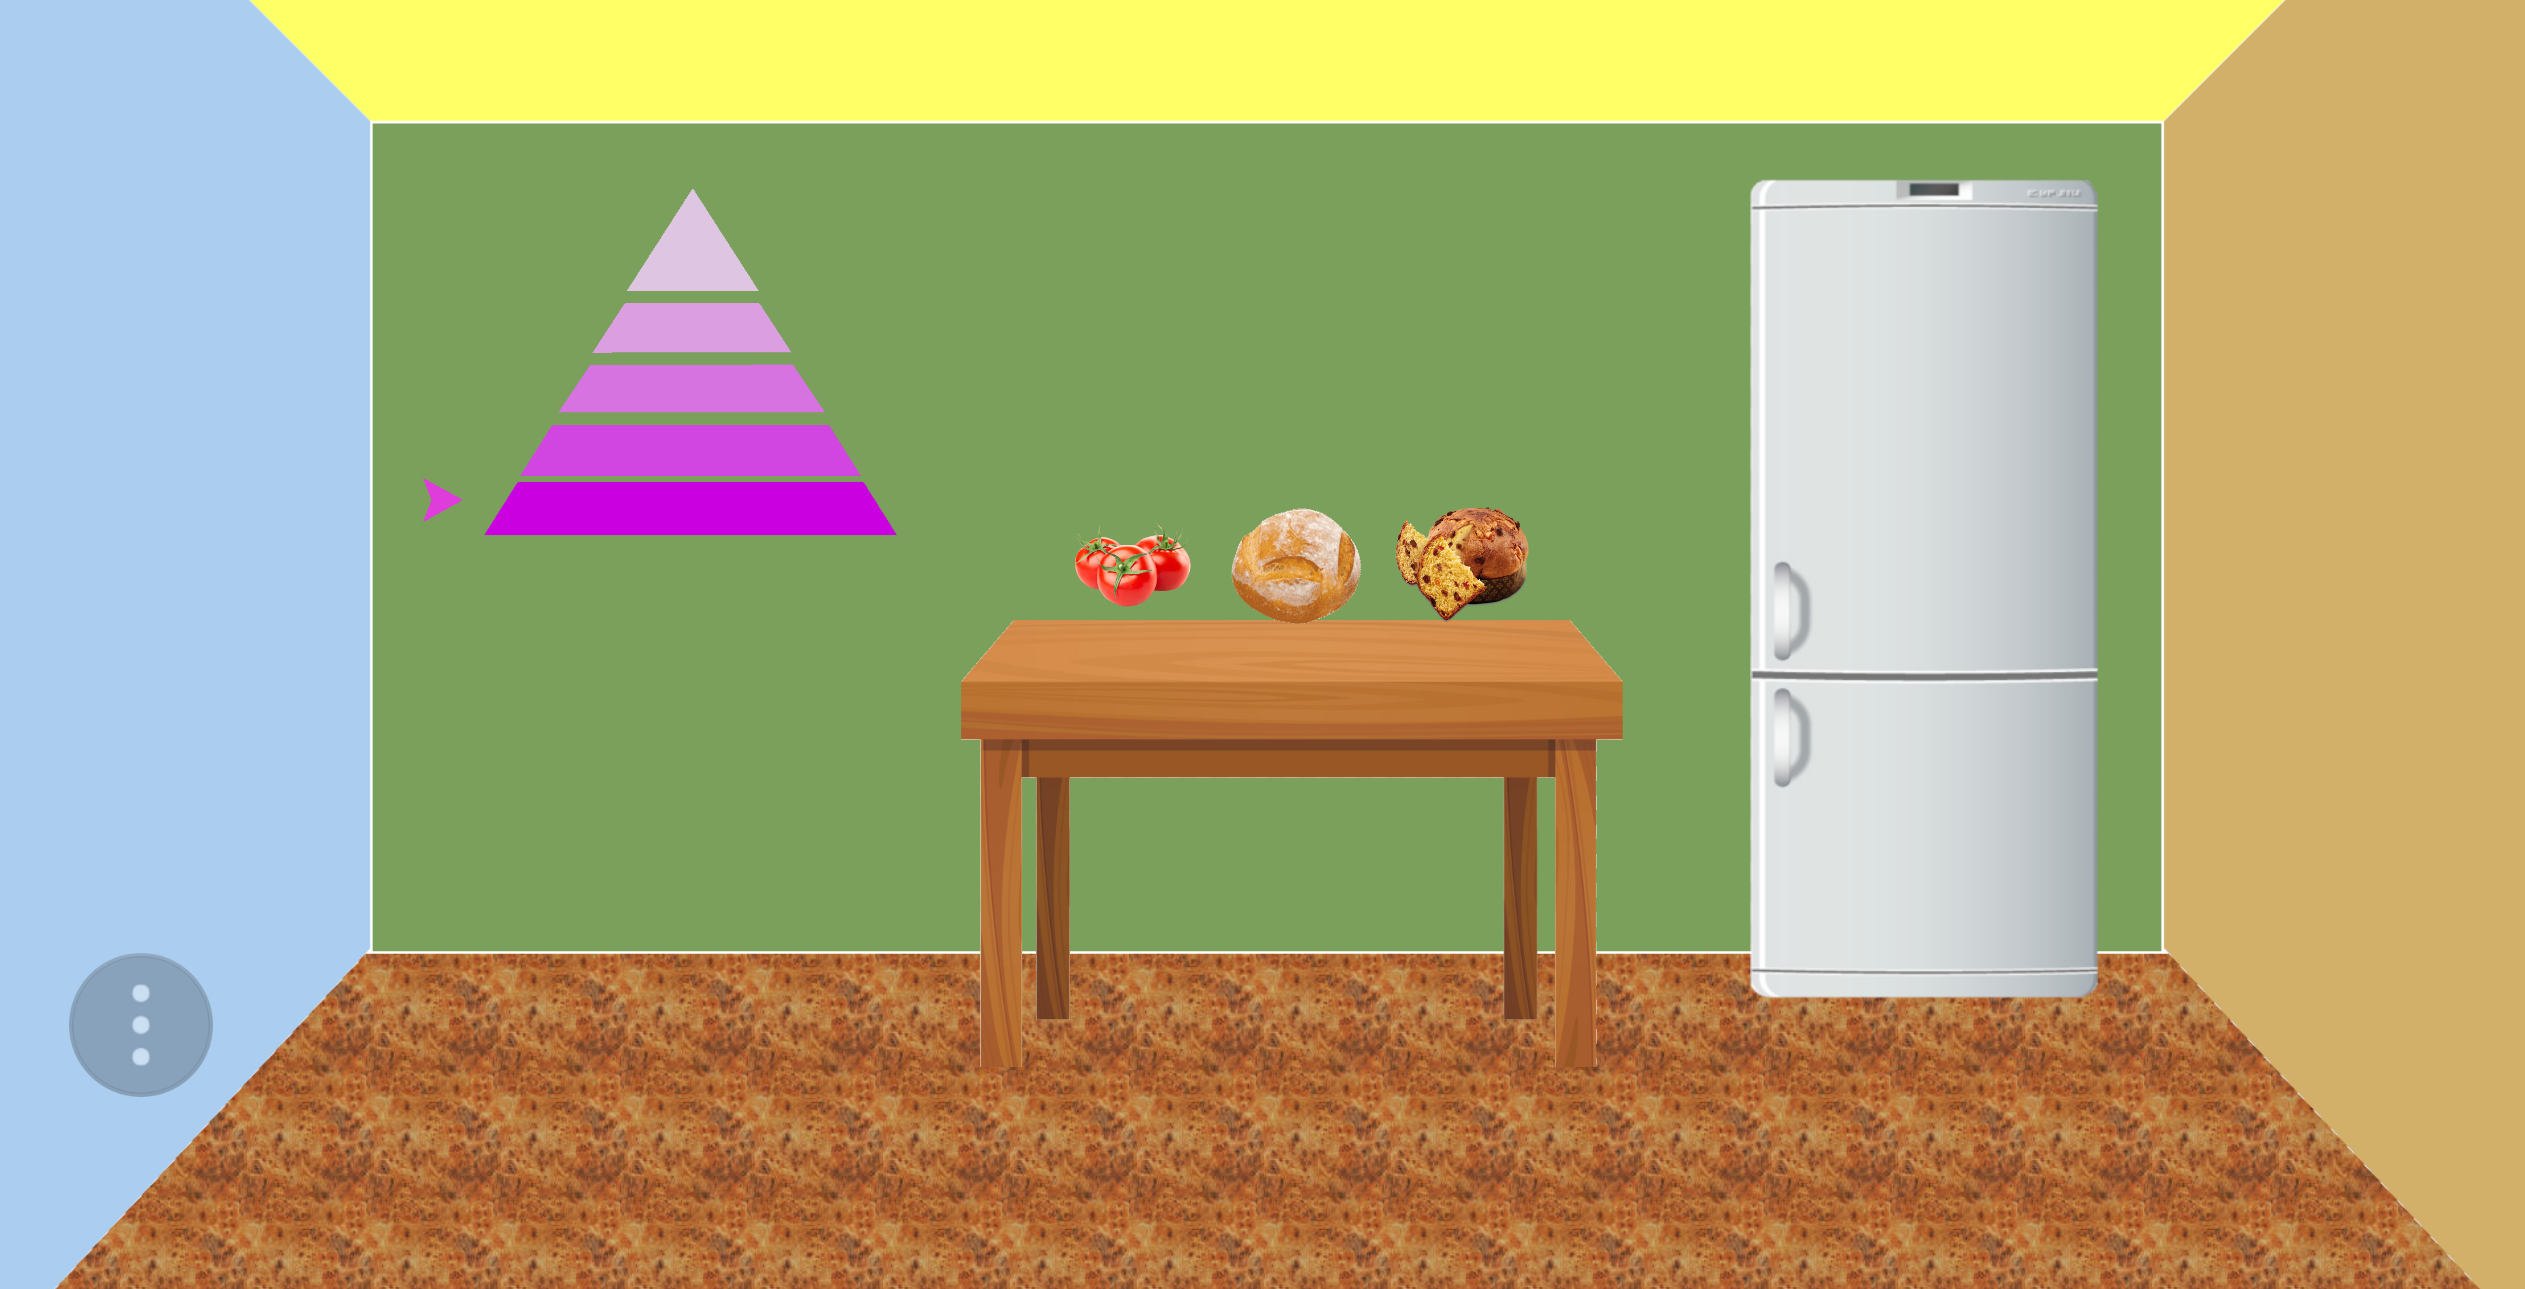
\includegraphics[width=10cm, height=6cm]{immagini/newpyramid.png}
\caption{"Learn with the pyramid!" touchscreen page}\label{fig:newpyramid}
\end{figure}
\begin{figure}[H]
\centering
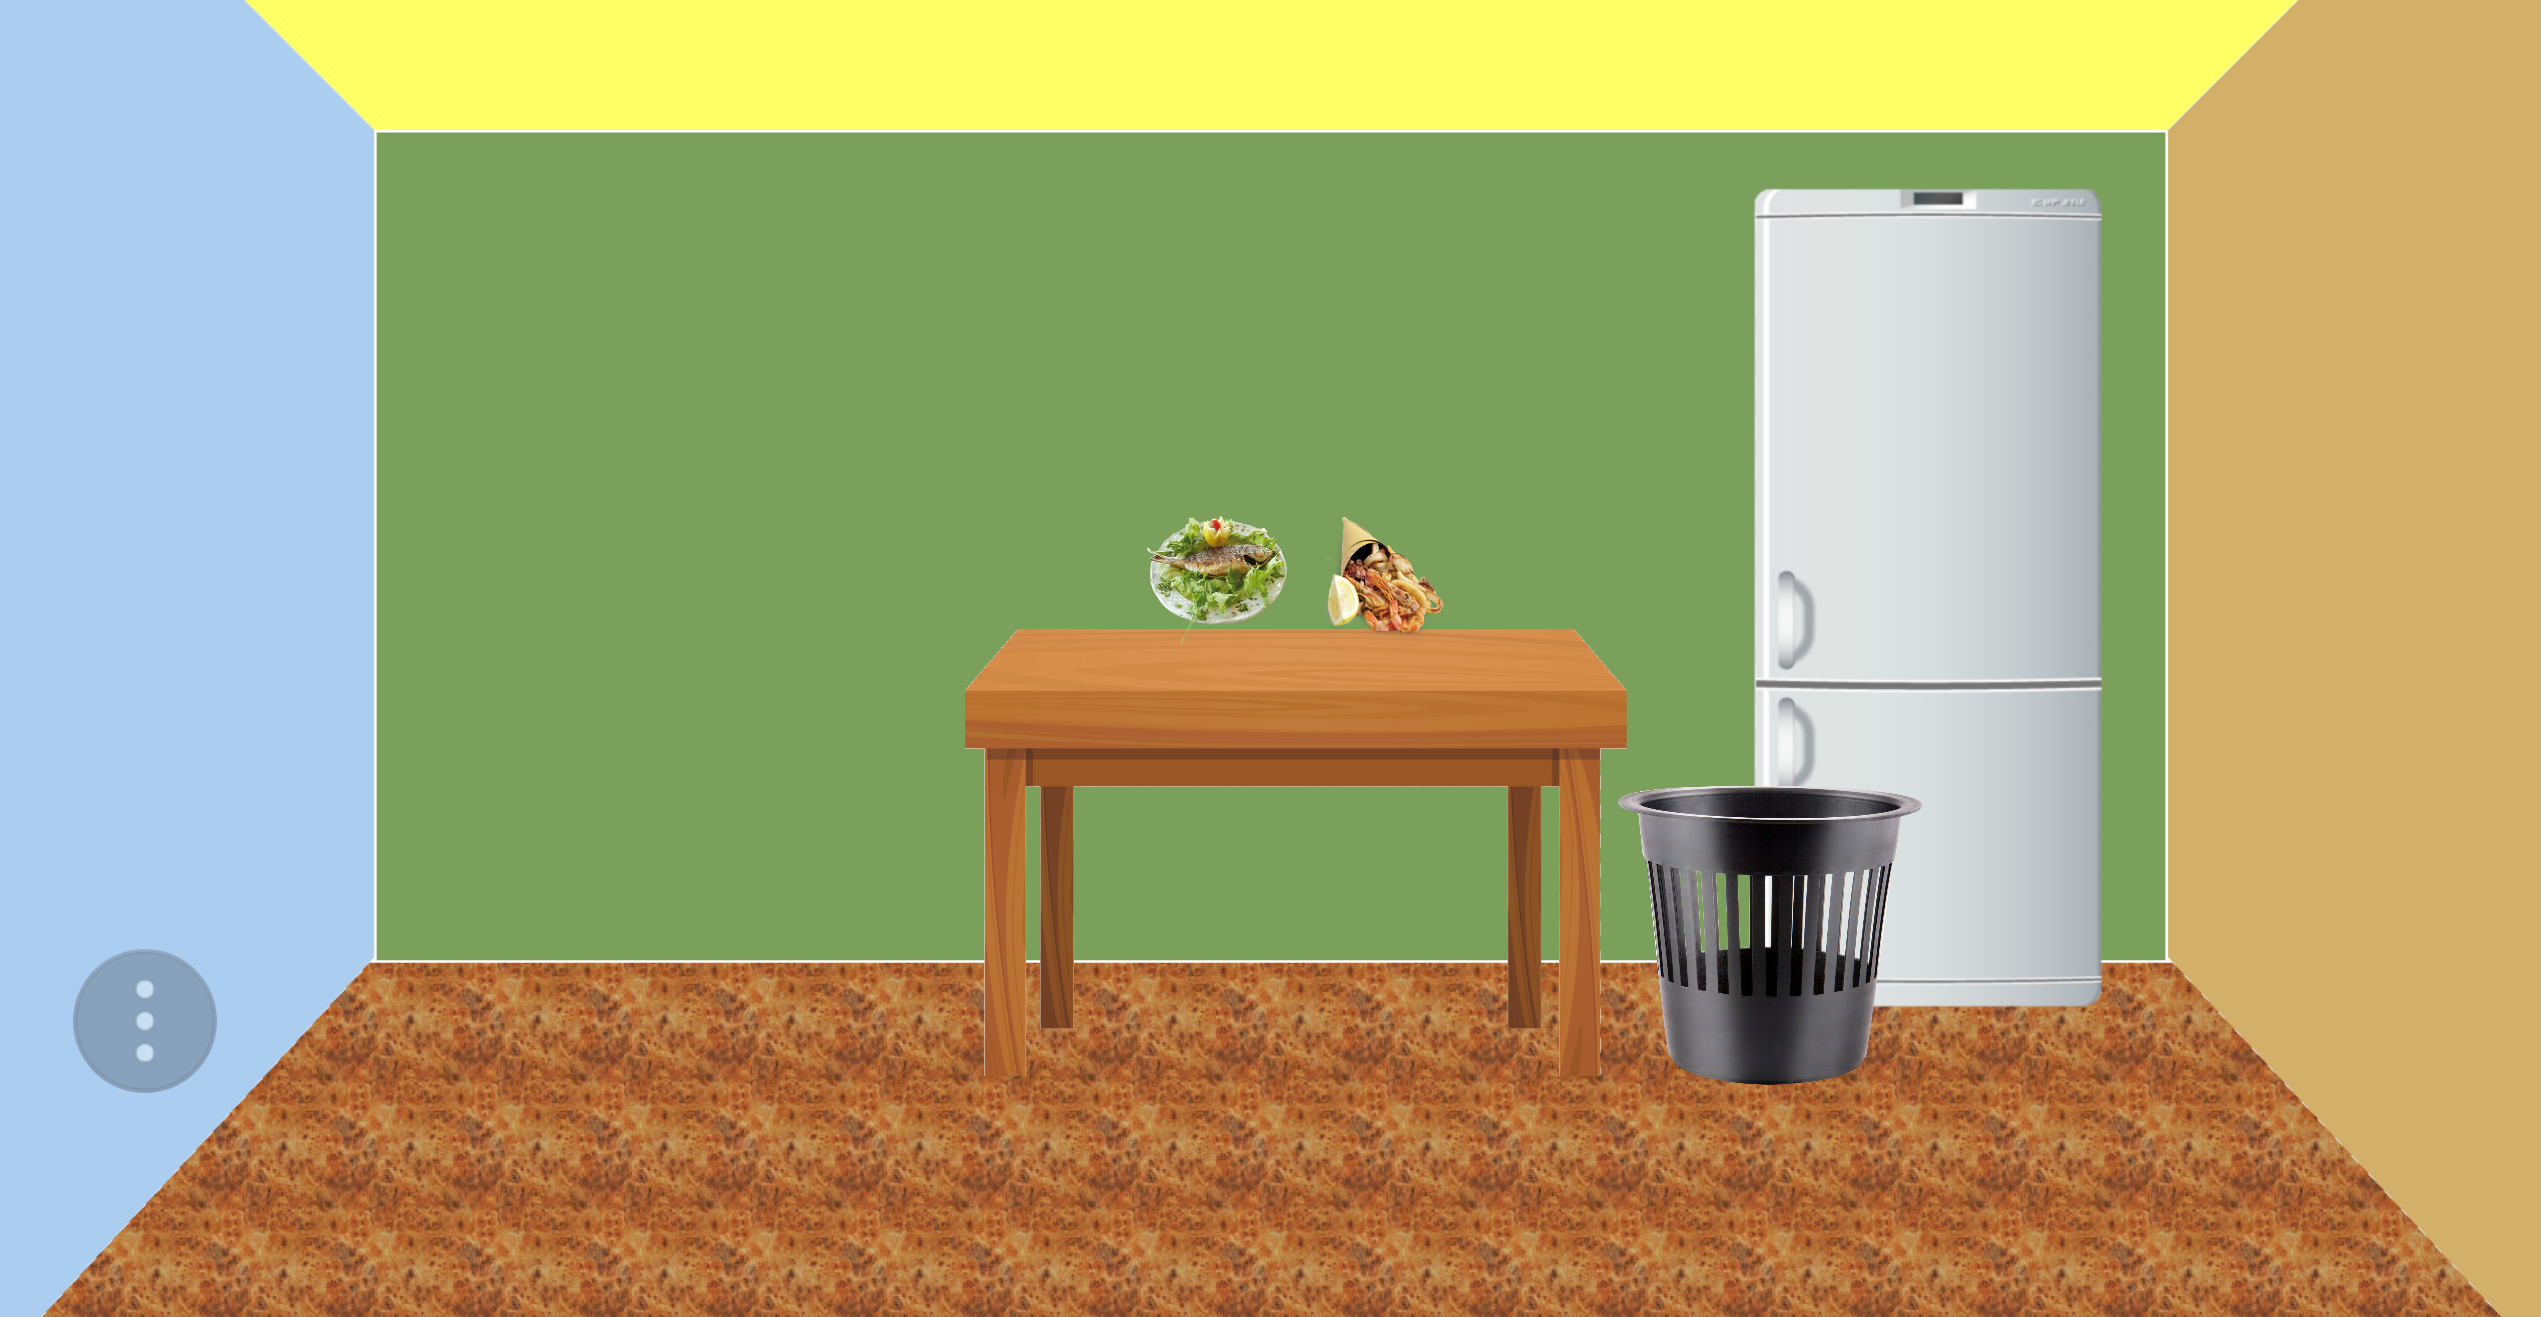
\includegraphics[width=10cm, height=6cm]{immagini/newhealthy.png}
\caption{"Healthy or not?" touchscreen page}\label{fig:newhealthy}
\end{figure}
\begin{figure}[H]
\centering
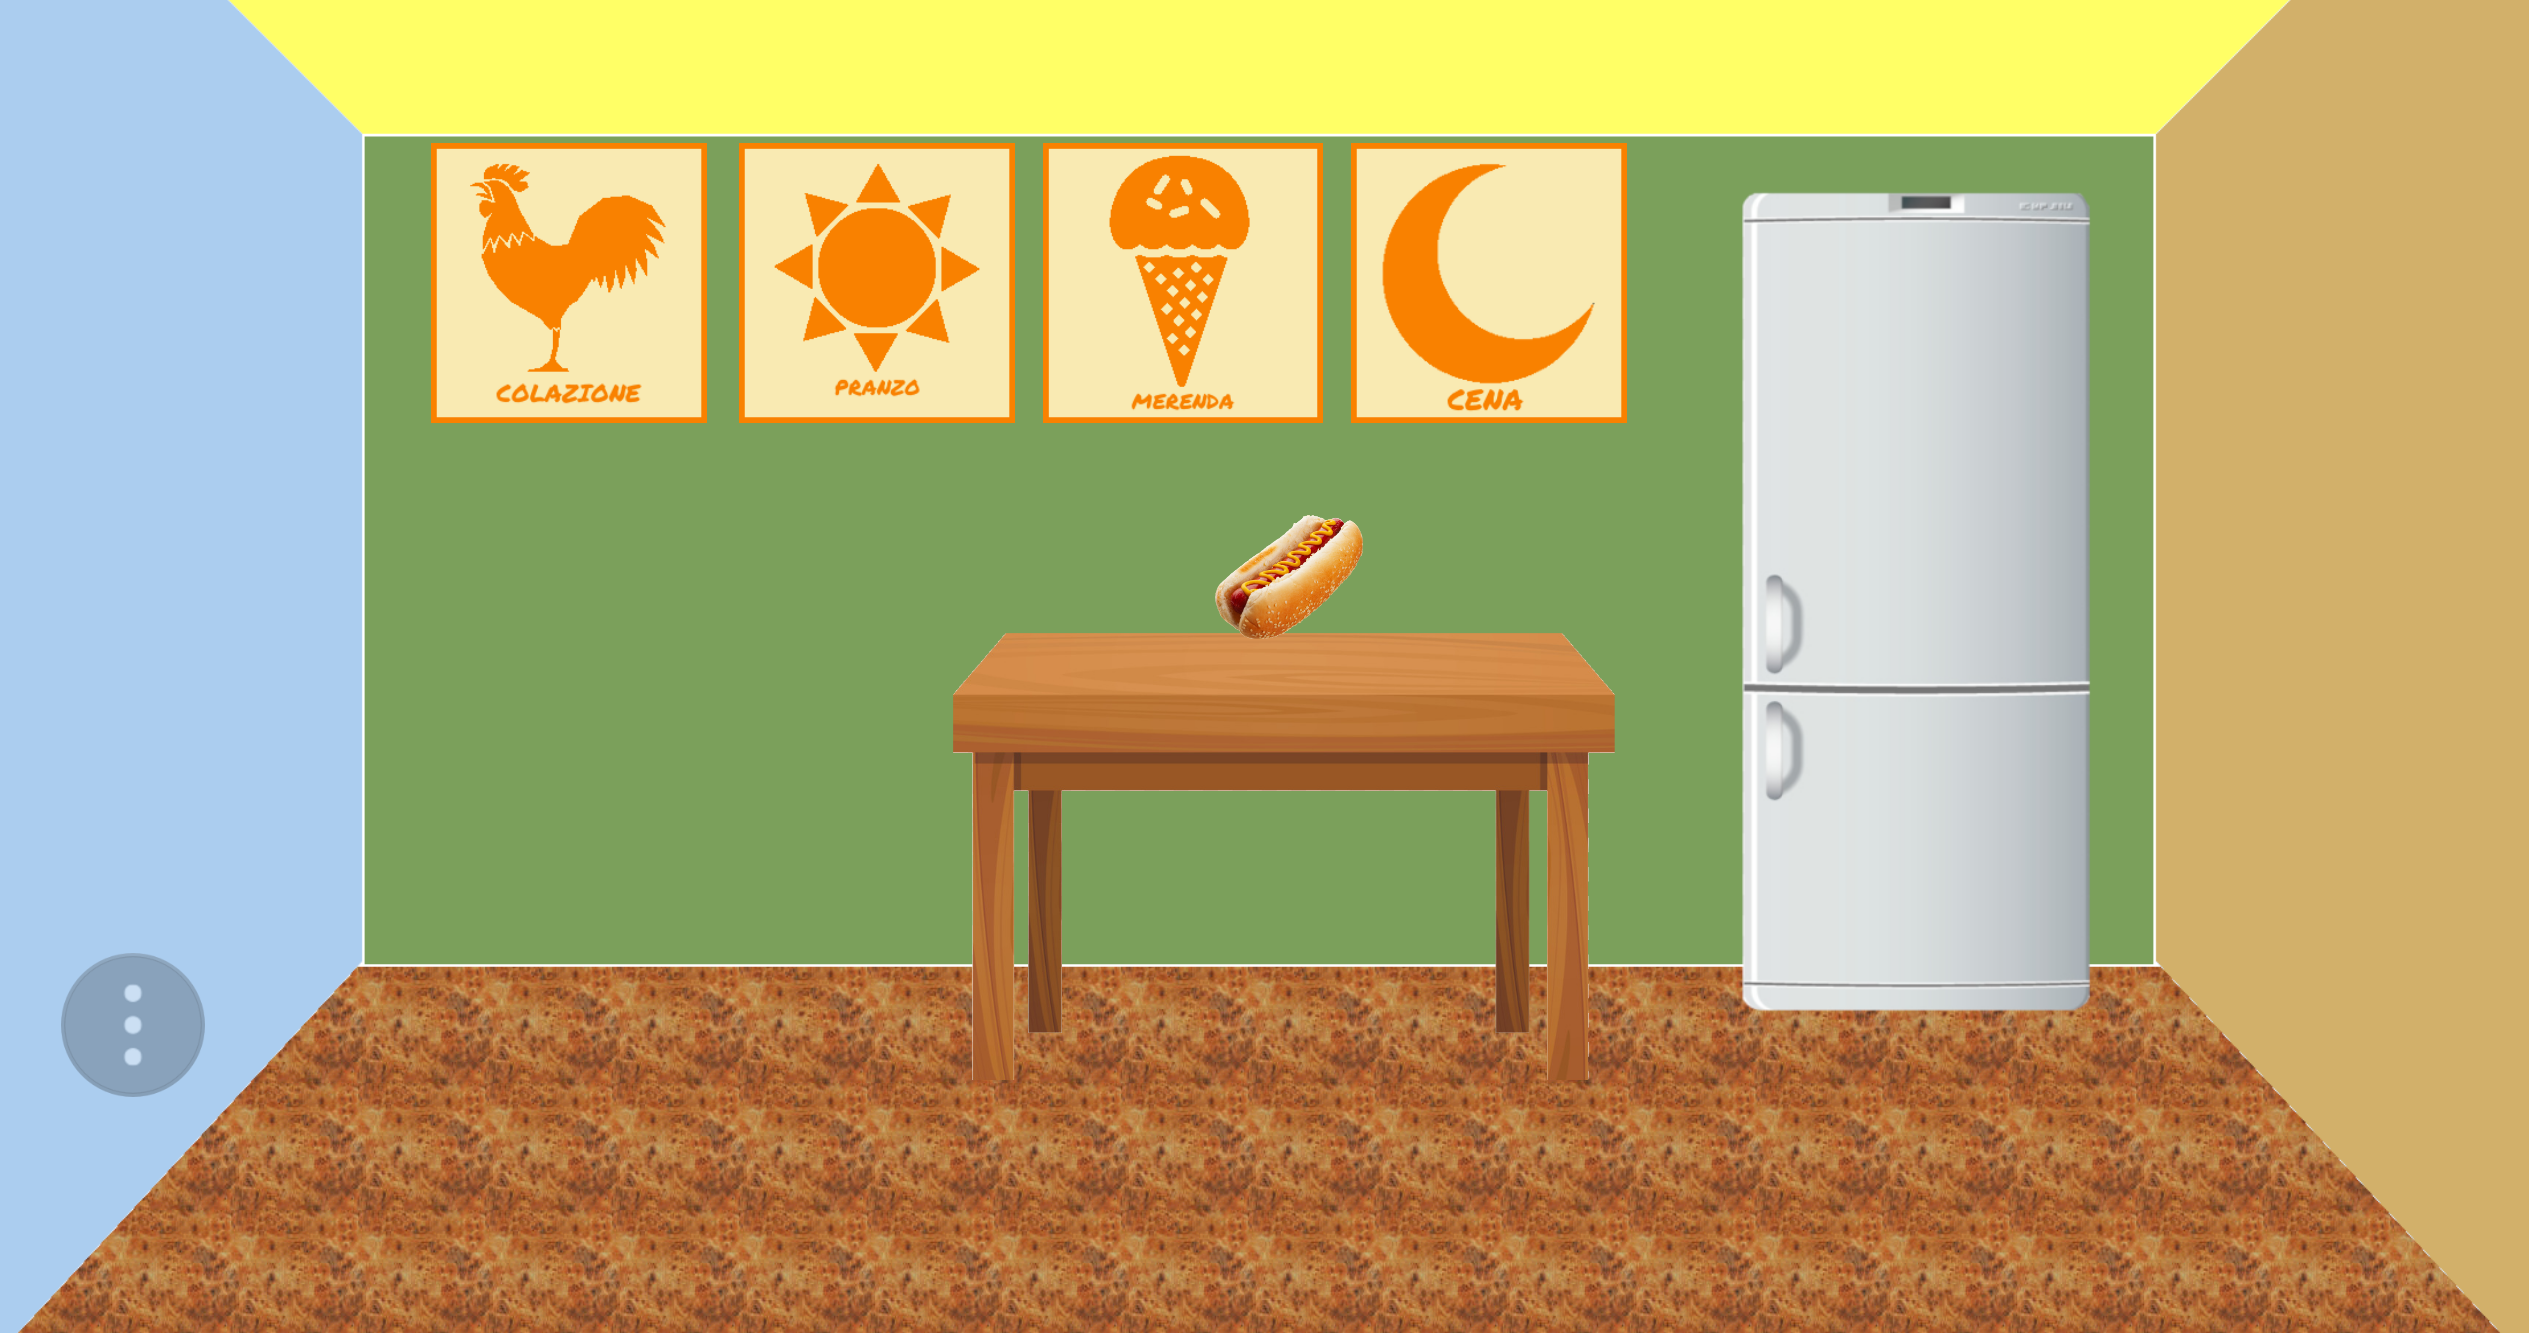
\includegraphics[width=10cm, height=6cm]{immagini/newlet.png}
\caption{"Let's eat!" touchscreen page}\label{fig:newlet}
\end{figure}
\section{Allergy game}
\section{Other modifications}